\newpage
\clearpage

\section{Proposta de Segmentação Panóptica em Componentes Visuais}
\label{proposal:proposal}

Considerando as segmentações modernas citadas nos Capítulos \ref{semantic:semantic}, \ref{instance:instance} e \ref{panoptic:panoptic}, fica claro que a segmentação panóptica é nomeada como a que possui maior riqueza de detalhes, de modo a ter uma compreensão mais clara das cenas, todavia considerando os problemas discorridos no Capítulo \ref{panoptic:panoptic}, bem como na Seção \ref{panoptic:conclusion} estudos vêm sendo desenvolvidos para solucionar esses obstáculos.

\begin{sloppypar}
Dentre os estudos desenvolvidos, cita-se o de Part-Aware Panoptic Segmentation \cite{DeGeus2021} com as propostas de trazer uma visão holística maior para as cenas e unir tarefas de \textit{scene parsing} e \textit{part parsing}, dispondo-se, indiretamente, também a trabalhar com objetos de pequena escala.
\end{sloppypar}

Dentre as áreas com oportunidades para o desenvolvimento e aplicação dessa técnica, a qual ainda não fora explorada, cita-se a área odontológica que, como também citado na Introdução (Capítulo \ref{intro:intro}), possibilita desafios com a meta de descrever o que há na boca a partir de fotografias orais, o que pode ser explorado por meio de um \textit{framework} de segmentação panóptica.

Sendo assim, este trabalho tem como objetivo aplicar técnicas de segmentação panóptica em componentes visuais odontológicos de modo a obter as segmentações organizada hierarquicamente, ou seja, com os segmentos de cada pixel nas cenas e suas partes, o que é exemplificado por meio da Figura \ref{proposal:proposal:fig:3}. Além disso, tem a nova proposta para a aplicação \textit{pooling} nos modelos base, com o intuito de buscar resultado relevantes no que se refere às validações de segmentação panóptica.

\begin{figure}[H]
    \centering
    \caption{Exemplo de aplicação de \textit{Part-Aware Panoptic Segmentation}.}
    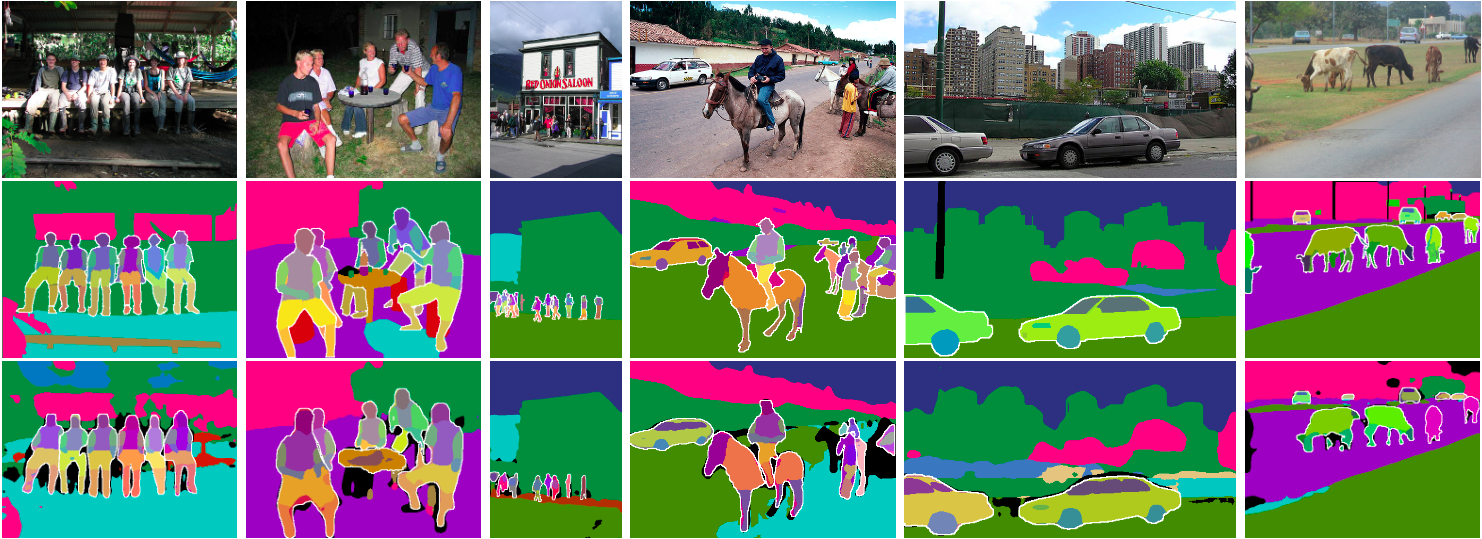
\includegraphics[width=1\linewidth]{recursos/imagens/proposal/part-aware-example.png}
    \label{proposal:proposal:fig:3}
    {\tiny Linhas contendo a imagem de entrada, valor de referencia e segmentação realizada com o método \textit{part-aware}, respectivamente, de cima para baixo.}

    \vspace*{1 cm}
    Fonte: \cite{DeGeus2021}.
\end{figure}

Em resumo, dentre as perspectivas de contribuição deste trabalho, lista-se:

\begin{enumerate}[I]
  \item A utilização da segmentação panóptica para a segmentação de componentes visuais na área odontológica;
  \item A disponibilização do código de maneira \textit{open source} com a finalidade de dar suporte aos trabalhos na área de \textit{part-aware panoptica segmentation}.
  \item A avaliação e adaptação (caso necessário) de uma ferramenta que auxilie a anotação de imagens com técnicas de segmentação;
  \item A aplicação da técnica \textit{block-based pca} na camada de \textit{pooling} dos modelos base para a segmentação panóptica.
\end{enumerate}

As demais seções desse capítulo estão organizadas de seguinte modo que a Seção \ref{proposal:matmet} descreve sobre os materiais e métodos utilizados nos experimentos, a Seção \ref{proposal:methodology} descreve a metodologia utilizada em alguns dos experimentos propostos, a Seção \ref{proposal:cron} apresenta um cronograma das atividades neste trabalho, e, finalmente, a Seção \ref{proposal:expres} demonstra alguns resultados esperados no decorrer do andamento do presente trabalho.


\subsection{Materiais e Métodos}
\label{proposal:matmet}
Nesta Seção, serão discorridos os detalhes sobre as tecnologias que serão utilizadas para o desenvolvimento de um modelo de segmentação panóptica que segmenta componentes visuais (Subseção \ref{proposal:tec}), sobre os conjuntos de dados e as estratégias utilizadas para cumprirem com o objetivo da segmentação (Subseção \ref{proposal:dataset}) e, por fim, as técnicas e métodos escolhidos para serem utilizados nos experimentos (Subseção \ref{proposal:method}).


\subsubsection{Tecnologias}
\label{proposal:tec}
Dentre as tecnologias planejadas para o desenvolvimento do presente trabalho, vale citar que destaca-se o uso da linguagem de programação interpretada e de alto nível, \textit{Python}, sendo essa uma linguagem vantajosa por ser popularmente conhecida em meio cientifico, com uma ampla comunidade e com  bibliotecas dispostas para facilitar o desenvolvimento de soluções \cite{Millman2011PythonEngineers}.

Já em relação às bibliotecas planejadas ao projeto, destacam-se aquelas cujo desenvolvimento é amplamente utilizado para o auxilio de projetos de visão computacional, aprendizado de máquina e redes neurais, das quais cita-se: \textit{PyTorch}, \textit{Keras}, \textit{TensorFlow}, \textit{OpenCV}, \textit{Numpy}, \textit{Pandas}, entre outras, dando destaque para a biblioteca \textit{Detectron2} \cite{detectron2} que já possui algumas funções especializadas para o trabalho com segmentações, incluindo redes de segmentação panóptica.

Por fim, em relação aos métodos desenvolvido para cumprir com os objetivos do presente trabalho, no que lhes concerne, de realizar a segmentação de componentes visuais, declara-se que serão disponibilizado de modo \textit{Open Source} por meio do \textit{Github} do autor\footnote{Perfil \textit{Github} do autor – \url{https://github.com/Lucs1590}}, segundo os preceitos a licença Apache v2.0 \cite{Licenses}, com o intuito de contribuir com o crescimento de futuros pesquisadores, além de possibilitar futuras melhorias da aréa de segmentação com uso de segmentação hierárquica.


\subsubsection{Conjuntos de Dados}
\label{proposal:dataset}
Em relação ao conjunto de dados, ressalta-se que foi estabelecido uma parceria com a Faculdade de Odontologia de Araraquara - UNESP, de modo que ...

\subsubsection{Método}
\label{proposal:method}

\subsection{Metodologia}
\label{proposal:methodology}

\subsubsection{Transferência de Aprendizado}
\label{proposal:transf}

\subsubsection{Avaliação}
\label{proposal:avaliation}

O método de avaliação escolhido seguiu no mesmo caminho do artigo tomado como referência para realizar a segmentação \textit{part-aware panoptic segmentation} \cite{DeGeus2021}, que, no que lhe concerne, teve como base o artigo pioneiro de segmentação panóptica \cite{Kirillov2019a}, que aplica a métrica PQ (Equação \ref{panoptic:eq:2}), realizando uma sucinta adaptação que possibilita metrificar as partes das segmentações panópticas visto que é aplicado para cada uma das classes ($l$) presentes na cena, sendo elas \textit{thing} ou \textit{stuff}. Através da equação \ref{proposal:avaliation:eq:1} é possível entender a métrica de avaliação \textit{Part-PQ}, a qual fora escolhida para avaliação.

\begin{equation}
\label{proposal:avaliation:eq:1}
    PartPQ = \frac{\sum _{(p,g) \in VP} IoU_p(p,g)}{|VP|+ \frac{1}{2}|FP| + \frac{1}{2}|FN|}.
\end{equation}

Em relação à Equação \ref{proposal:avaliation:eq:1}, destaca-se ainda que a segmentação das partes dentro de um segmento é capturada principalmente por meio do termo $IoU_p(p,g)$, sendo que no termo é aplicado um condicional com o intuito de deixar a classe segmentada com parte ($\mathcal{L}^{parts}$) e sem partes ($\mathcal{L}^{no-parts}$) dentro das mesmas condições, ou seja, para as classes com partes presentes, aplica-se a métrica de $mIoU$ para cada pixel de parte dentro de um segmento, enquanto para segmentações sem partes, aplica-se a $IoU$ que comumente é utilizada na métrica PQ (Equação \ref{panoptic:eq:2}). O condicional supracitado da-se por meio da seguinte expressão:

\begin{equation}
\label{proposal:avaliation:eq:2}
    IoU_p(p,g)= \left\{\begin{matrix}
        mIoU_{part}(p,g), & l \in \mathcal{L}^{parts}    & \\ 
        IOU_ins(p,g),        & l \in \mathcal{L}^{no-parts} & 
    \end{matrix}\right.
\end{equation}

Por fim, após a aplicação de PartPQ em todas as classes, calcula-se a média entre avaliações realizadas, de modo que é possível avaliar o desempenho do modelo em toda a cena e demonstrou resultados consideráveis quando comparado à métrica original \cite{DeGeus2021}.

\subsection{Revisão de Literatura}
\label{proposal:revision}

Em meio a vários estilos de revisão, vale dizer que a revisão sistemática é amplamente difundida em meio cientifico, destacando-se em pesquisas de âmbito clínico e médico e garantindo menos viés, maior confiabilidade e um resumo de forma crítica dos trabalhos científicos \cite{barbosa2019}. Sendo assim, no presente trabalho, foi realizado uma revisão, bem como buscas baseadas nos artigos \cite{barbosa2019} e \cite{liberati2009}, de modo que se inspirou nas recomendações dos mesmos, salvo os casos relacionados a questões de aplicações clínicas.

Em relação às revisões, foram realizadas duas, de modo a abranger tanto os artigos técnicos em relação à segmentação panóptica, quanto artigos que servissem de base para a segmentação na área odontológica. A questão a ser tomada como base para esse estudo é: Como modelar \textit{framework} para segmentar imagens de componentes visuais hierarquicamente?

Para a primeira revisão citada, foram procurados todo tipo de estudo publicados a partir do ano de 2019 até o ano presente (2022) com o assunto relacionado a \textit{panoptic segmentation}, de modo a se basear no ano de publicação do artigo pioneiro \cite{Kirillov2019a} no assunto. Foram usados os termos a seguir em diferentes combinações: ``\textit{panoptic segmentation}'', ``\textit{part}'' e ``\textit{part-aware}''. Os idiomas foram restritos à português e inglês.

Os critério de inclusão baseou-se em artigos que possuíssem a citação da técnica de segmentação \textit{part-aware} de modo a contribuir com uma segmentação hierárquica dos componentes que compunham a cena. Já em relação aos critérios de exclusão destaca-se artigos com descrição inadequada das variáveis de interesse a esta revisão, quando o artigo era especifico para uma determinada aplicação que não condizia com o tema (como carros autônomos), quando o estudo estava duplicado entre as ferramentas de busca e quando as variáveis não eram de interesse a esta revisão.

Sendo assim, os indicadores referentes as pesquisas realizadas sobre esse assunto podem ser visualizadas no diagrama abaixo (Figura \ref{proposal:revision:fig:1}).

\begin{figure}[H]
    \centering
    \caption{Diagrama de revisão de estudos em segmentação panóptica.}
    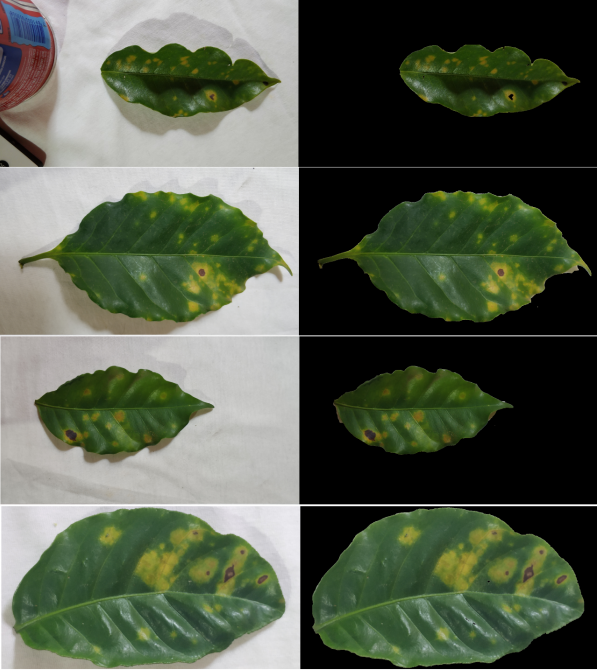
\includegraphics[height=2.3in]{recursos/imagens/introduction/grabcut.png}
    \label{proposal:revision:fig:1}

    \vspace*{1 cm}
    Fonte: do próprio autor.
\end{figure}

Quando se trata da segunda revisão em pauta, a que contempla as segmentações na área odontológica, destaca-se que os estudos procurados também não se limitaram ao tipo, incluindo congressos, artigos de revista, entre outros, além de utilizarem o intervalo dos anos de 2019 a 2022 como métrica, de modo a encontrar segmentações odontológicas que acompanhasse a técnica de segmentação panóptica. Os termos utilizados estão listados a seguir, de modo que foram buscados em diferentes combinações: ``odonto'', ``\textit{dentistry}'', ``\textit{deep learning}'', ``\textit{semantic segmentation}'', ``\textit{instance segmentation}'', ``\textit{panoptic segmentation}'' e ``CNN''. Os idiomas foram restritos à português e inglês.

Quanto aos critérios de inclusão, destaca-se os artigos que abordaram ao menos uma das segmentações modernas, de feitio a estarem alinhados com a proposta do projeto. Quanto aos critérios de exclusão, pode-se dizer que são similares aos da primeira revisão, relatando artigos com descrição inadequada das variáveis de interesse, estudos duplicados entre as ferramentas de busca e quando as variáveis não eram de interesse a esta revisão. Dessa forma, por meio da Figura \ref{proposal:revision:fig:2} é possível visualizar a representação da revisão realizada.

\begin{figure}[H]
    \centering
    \caption{Diagrama de revisão de estudos em segmentação panóptica.}
    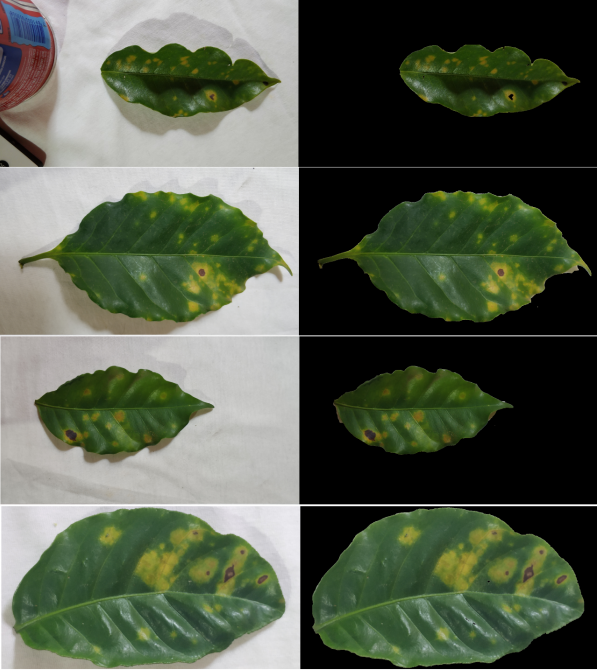
\includegraphics[height=2.3in]{recursos/imagens/introduction/grabcut.png}
    \label{proposal:revision:fig:2}

    \vspace*{1 cm}
    Fonte: do próprio autor.
\end{figure}
.

\subsection{Cronograma}
\label{proposal:cron}

Com o intuito de listar todas as atividades necessárias para o cumprimento do projeto, bem como definição do período em que as mesmas devem ser realizadas, foram construídas a Tabela \ref{proposal:cron:table:1} e \ref{proposal:cron:table:2}, almejando realizar no máximo quatro  experimentos simultaneamente, considerando a complexidade, esforço e incerteza envolvida em cada um desses testes. Em relação às submissões é desejado realizar uma para conferência, objetivando  contribuir com os experimentos desenvolvidos na primeira etapa e uma segunda para um periódico com o intuito de contribuir com as descobertas realizadas no experimento IV. Por fim, tem se como objetivo realizar a escrita do trabalho em todo o período do cronograma - salvo o mês planejado para a defesa - sendo que essa atividade ocorrera paralelamente aos demais experimentos e atividades listadas.

\definecolor{midgray}{gray}{.5}

\begin{table}[H]
    \centering
    \caption{Atividades a serem desenvolvidas.}
    \label{proposal:cron:table:1}
    \resizebox{\textwidth}{!}{
        \begin{tabular}{l|l}
            \textbf{Índice} & \textbf{Descrição}                                                                                                             \\ \hline
            I - 1           & Obtenção e anotação de imagens odontológicas para o treinamento e teste da rede.                                               \\
            I - 2           & Aplicação da biblioteca \textit{Detectron2} para realização de segmentação panóptica.                                          \\
            I - 3           & Modelagem da rede com o uso de \textit{part-aware panoptic segmentation}, segundo sugerido por \cite{DeGeus2021}.              \\
            I - 4           & Submissão de testes na rede modelada, com o intuito de saber como a rede tem performado.                                       \\
            II - 1          & Avaliar e adaptar (caso necessário) uma ferramenta que auxilie a anotação de imagens;                                          \\
            III - 1         & Desenvolvimento de biblioteca \textit{open source} com métodos que auxiliam a segmentação hierárquica de componentes visuais.  \\
            IV - 1          & Transferência de aprendizado entre os conjuntos de dados disponíveis e conjunto de dado anotado.                               \\
            IV - 2          & Modificação da arquitetura base para aplicação de \textit{block-based PCA} na camada de \textit{pooling};                      \\
            V - I           & Desenvolvimento de métodos de visualização da informação para comparar os conjuntos de dados e as métricas das redes.          \\
            V - II          & Comparação de rede de segmentação panóptica com a rede desenvolvida.                                                 
        \end{tabular}
    }

    \vspace*{1 cm}
    Fonte: do próprio autor.
\end{table}


\begin{table}[ht]
    \centering
    \caption{Cronograma de atividades.}
    \label{proposal:cron:table:2}
        \begin{tabular}{|c|c|c|c|c|c|c|l|l|} 
            \hline
                                    & \multicolumn{8}{c|}{2022}                        \\ 
            \hline
            \textbf{Macroatividades}        & FEV & MAR & ABR & MAI & JUN & JUL & AGO & SET  \\ 
            \hline
            Experimento I                   & \cellcolor{midgray} & \cellcolor{midgray} & \cellcolor{midgray} &     &     &     &     &      \\ 
            \hline
            Experimento II                 &     & \cellcolor{midgray} & \cellcolor{midgray} &     &     &     &     &      \\ 
            \hline
            Experimento III                  &     &     &     & \cellcolor{midgray} & \cellcolor{midgray} & \cellcolor{midgray} &     &  \\ 
            \hline
            Experimento IV                  &     &     &     & \cellcolor{midgray} & \cellcolor{midgray} &     &     &      \\ 
            \hline
            Experimento V                   &     &     &     &     &     & \cellcolor{midgray} &     &      \\ 
            \hline
            Escrita da dissertação          & \cellcolor{midgray} & \cellcolor{midgray} & \cellcolor{midgray} & \cellcolor{midgray} & \cellcolor{midgray} & \cellcolor{midgray} & \cellcolor{midgray} &  \\ 
            \hline
            Submissão para conferência      &     &     &     & \cellcolor{midgray} &     &     &     &      \\ 
            \hline
            Submissão para periódico        &     &     &     &     &     &     & \cellcolor{midgray} &      \\ 
            \hline
            Defesa                          &     &     &     &     &     &     &     & \cellcolor{midgray} \\
            \hline
        \end{tabular}
    
    \vspace*{1 cm}
    Fonte: do próprio autor.
\end{table}

\subsection{Resultados Esperados}
\label{proposal:expres}